\documentclass[tikz,border=10pt]{standalone}
\usepackage[T1]{fontenc}
\usepackage{helvet}
\renewcommand{\familydefault}{\sfdefault}
\usepackage{tikz}
\usetikzlibrary{arrows.meta,positioning,shapes.multipart,shapes.geometric,fit,backgrounds,calc,shadows}

\definecolor{navy}{HTML}{1F3A5F}
\definecolor{teal}{HTML}{0C6B58}
\definecolor{amber}{HTML}{D9822B}
\definecolor{crimson}{HTML}{B42318}
\definecolor{violet}{HTML}{6B21A8}
\definecolor{sky}{HTML}{2186EB}
\definecolor{slate}{HTML}{486581}
\definecolor{mist}{HTML}{F0F4F8}
\definecolor{line}{HTML}{9FB3C8}

\tikzset{
  >={Stealth[length=2.6mm]},
  box/.style={draw=navy, very thick, rounded corners=3pt, fill=white, align=center,
    inner sep=5pt, font=\small, minimum height=9mm},
  softbox/.style={box, draw=slate, thick, fill=mist},
  layer/.style={draw=line, dashed, rounded corners=6pt, inner sep=7pt},
  layertitle/.style={font=\bfseries\small, text=slate, anchor=north west},
  flow/.style={->, thick, draw=navy},
  dflow/.style={->, thick, draw=slate, dashed},
  lbl/.style={font=\scriptsize, text=slate, fill=white, inner sep=1.5pt},
  umlclass/.style={draw=navy, thick, fill=white, rectangle split, rectangle split parts=3,
    rectangle split part fill={navy!12,white,white}, align=left, font=\scriptsize,
    inner sep=3pt, text width=#1},
  umlclass/.default=38mm,
}

\tikzset{
  comp/.style={{Diamond[fill=navy,length=3.2mm,width=2.2mm]}-, thick, draw=navy},
  agg/.style={{Diamond[open,fill=white,length=3.2mm,width=2.2mm]}-, thick, draw=navy},
  real/.style={-{Triangle[open,fill=white,length=3mm,width=2.6mm]}, thick, dashed, draw=navy},
  gen/.style={-{Triangle[open,fill=white,length=3mm,width=2.6mm]}, thick, draw=navy},
  uses/.style={->, thick, dashed, draw=slate},
  mult/.style={font=\scriptsize, text=crimson},
}
\begin{document}
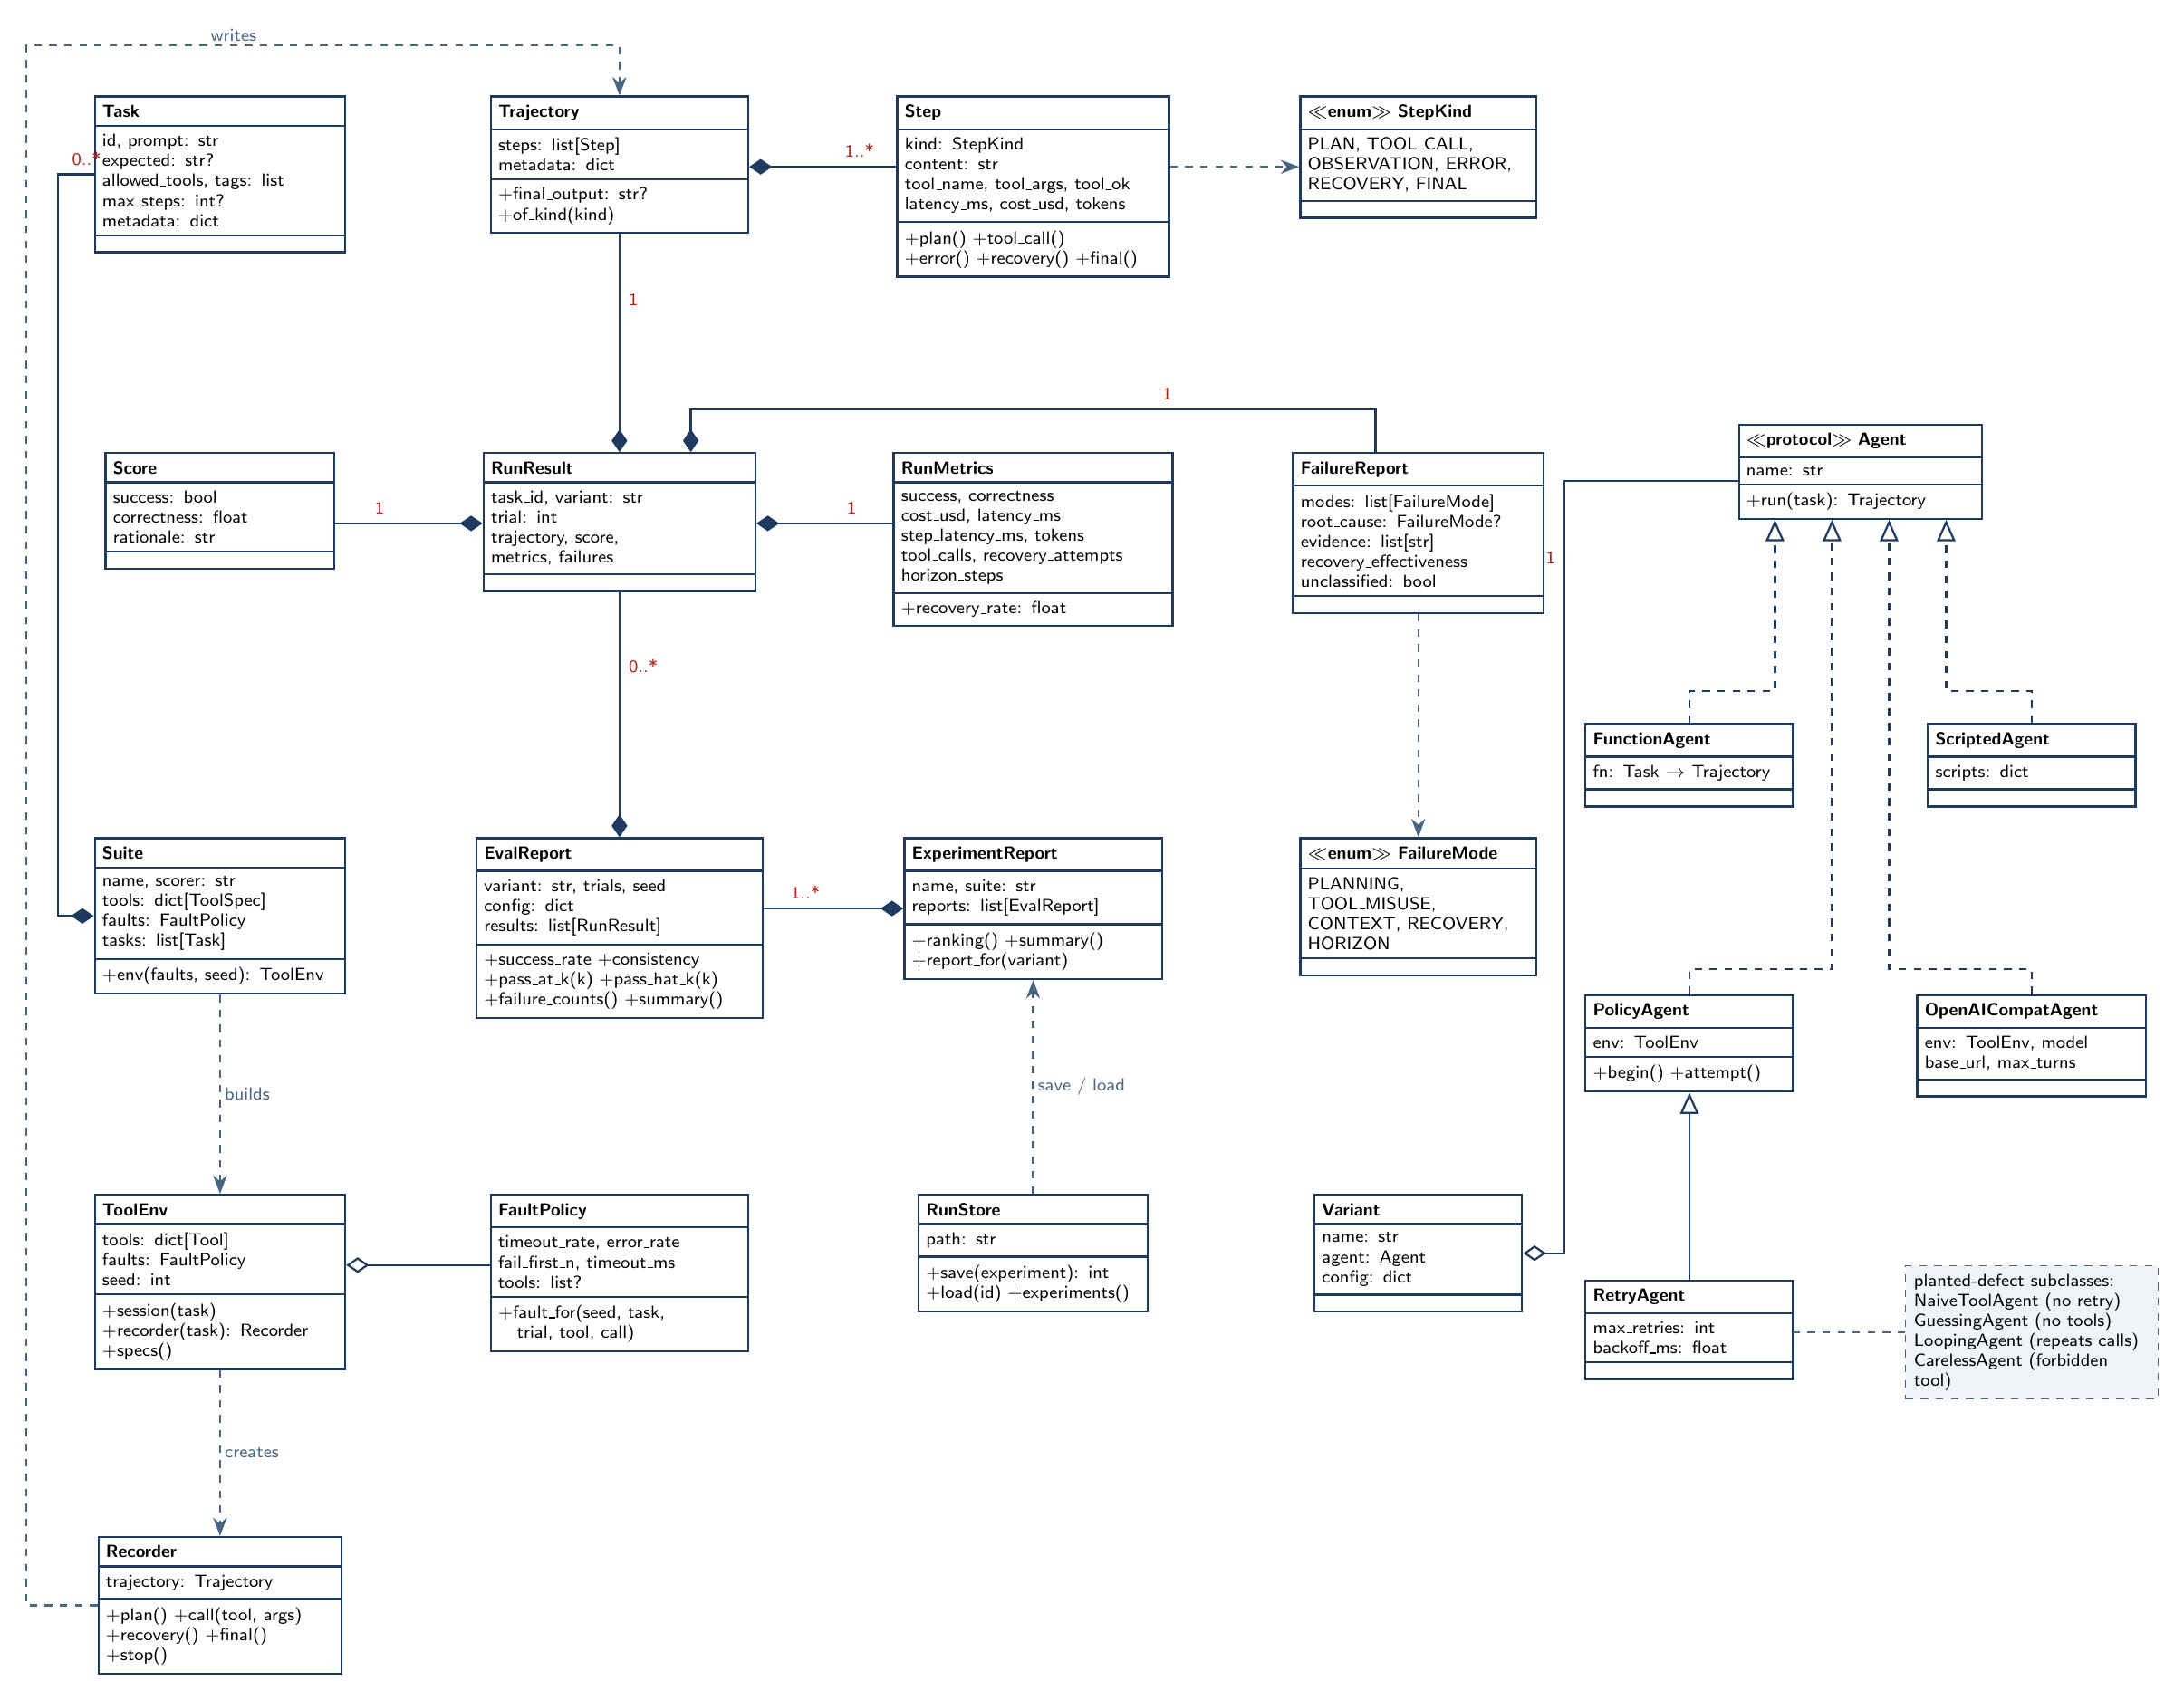
\begin{tikzpicture}[x=1cm,y=1cm]
  % Row 1: trajectory data
  \node[umlclass=33mm, anchor=north] (task) at (0,0) {\textbf{Task}
    \nodepart{second} id, prompt: str\\ expected: str?\\ allowed\_tools, tags: list\\ max\_steps: int?\\ metadata: dict
    \nodepart{third} };
  \node[umlclass=34mm, anchor=north] (traj) at (5.6,0) {\textbf{Trajectory}
    \nodepart{second} steps: list[Step]\\ metadata: dict
    \nodepart{third} +final\_output: str?\\ +of\_kind(kind)};
  \node[umlclass=36mm, anchor=north] (step) at (11.4,0) {\textbf{Step}
    \nodepart{second} kind: StepKind\\ content: str\\ tool\_name, tool\_args, tool\_ok\\ latency\_ms, cost\_usd, tokens
    \nodepart{third} +plan() +tool\_call()\\ +error() +recovery() +final()};
  \node[umlclass=31mm, anchor=north] (kind) at (16.8,0) {\textbf{$\ll$enum$\gg$ StepKind}
    \nodepart{second} PLAN, TOOL\_CALL,\\ OBSERVATION, ERROR,\\ RECOVERY, FINAL
    \nodepart{third} };

  % Row 2: one scored run
  \node[umlclass=30mm, anchor=north] (score) at (0,-5.0) {\textbf{Score}
    \nodepart{second} success: bool\\ correctness: float\\ rationale: str
    \nodepart{third} };
  \node[umlclass=36mm, anchor=north] (result) at (5.6,-5.0) {\textbf{RunResult}
    \nodepart{second} task\_id, variant: str\\ trial: int\\ trajectory, score,\\ metrics, failures
    \nodepart{third} };
  \node[umlclass=37mm, anchor=north] (metrics) at (11.4,-5.0) {\textbf{RunMetrics}
    \nodepart{second} success, correctness\\ cost\_usd, latency\_ms\\ step\_latency\_ms, tokens\\ tool\_calls, recovery\_attempts\\ horizon\_steps
    \nodepart{third} +recovery\_rate: float};
  \node[umlclass=33mm, anchor=north] (failure) at (16.8,-5.0) {\textbf{FailureReport}
    \nodepart{second} modes: list[FailureMode]\\ root\_cause: FailureMode?\\ evidence: list[str]\\ recovery\_effectiveness\\ unclassified: bool
    \nodepart{third} };

  % Row 3: reports and suites
  \node[umlclass=33mm, anchor=north] (suite) at (0,-10.4) {\textbf{Suite}
    \nodepart{second} name, scorer: str\\ tools: dict[ToolSpec]\\ faults: FaultPolicy\\ tasks: list[Task]
    \nodepart{third} +env(faults, seed): ToolEnv};
  \node[umlclass=38mm, anchor=north] (eval) at (5.6,-10.4) {\textbf{EvalReport}
    \nodepart{second} variant: str, trials, seed\\ config: dict\\ results: list[RunResult]
    \nodepart{third} +success\_rate +consistency\\ +pass\_at\_k(k) +pass\_hat\_k(k)\\ +failure\_counts() +summary()};
  \node[umlclass=34mm, anchor=north] (exp) at (11.4,-10.4) {\textbf{ExperimentReport}
    \nodepart{second} name, suite: str\\ reports: list[EvalReport]
    \nodepart{third} +ranking() +summary()\\ +report\_for(variant)};
  \node[umlclass=31mm, anchor=north] (mode) at (16.8,-10.4) {\textbf{$\ll$enum$\gg$ FailureMode}
    \nodepart{second} PLANNING, TOOL\_MISUSE,\\ CONTEXT, RECOVERY,\\ HORIZON
    \nodepart{third} };

  % Row 4: environment and storage
  \node[umlclass=33mm, anchor=north] (env) at (0,-15.4) {\textbf{ToolEnv}
    \nodepart{second} tools: dict[Tool]\\ faults: FaultPolicy\\ seed: int
    \nodepart{third} +session(task)\\ +recorder(task): Recorder\\ +specs()};
  \node[umlclass=34mm, anchor=north] (fault) at (5.6,-15.4) {\textbf{FaultPolicy}
    \nodepart{second} timeout\_rate, error\_rate\\ fail\_first\_n, timeout\_ms\\ tools: list?
    \nodepart{third} +fault\_for(seed, task,\\ \quad trial, tool, call)};
  \node[umlclass=30mm, anchor=north] (store) at (11.4,-15.4) {\textbf{RunStore}
    \nodepart{second} path: str
    \nodepart{third} +save(experiment): int\\ +load(id) +experiments()};
  \node[umlclass=27mm, anchor=north] (variant) at (16.8,-15.4) {\textbf{Variant}
    \nodepart{second} name: str\\ agent: Agent\\ config: dict
    \nodepart{third} };
  \node[umlclass=32mm, anchor=north] (rec) at (0,-20.2) {\textbf{Recorder}
    \nodepart{second} trajectory: Trajectory
    \nodepart{third} +plan() +call(tool, args)\\ +recovery() +final() +stop()};

  % Agents
  \node[umlclass=32mm, anchor=north] (agent) at (23,-4.6) {\textbf{$\ll$protocol$\gg$ Agent}
    \nodepart{second} name: str
    \nodepart{third} +run(task): Trajectory};
  \node[umlclass=27mm, anchor=north] (fn) at (20.6,-8.8) {\textbf{FunctionAgent}
    \nodepart{second} fn: Task $\rightarrow$ Trajectory
    \nodepart{third} };
  \node[umlclass=27mm, anchor=north] (scripted) at (25.4,-8.8) {\textbf{ScriptedAgent}
    \nodepart{second} scripts: dict
    \nodepart{third} };
  \node[umlclass=27mm, anchor=north] (policy) at (20.6,-12.6) {\textbf{PolicyAgent}
    \nodepart{second} env: ToolEnv
    \nodepart{third} +begin() +attempt()};
  \node[umlclass=30mm, anchor=north] (llm) at (25.4,-12.6) {\textbf{OpenAICompatAgent}
    \nodepart{second} env: ToolEnv, model\\ base\_url, max\_turns
    \nodepart{third} };
  \node[umlclass=27mm, anchor=north] (retry) at (20.6,-16.6) {\textbf{RetryAgent}
    \nodepart{second} max\_retries: int\\ backoff\_ms: float
    \nodepart{third} };
  \node[draw=slate, dashed, align=left, font=\scriptsize, text width=33mm, fill=mist, anchor=north] (subs) at (25.4,-16.4) {planted-defect subclasses:\\ NaiveToolAgent (no retry)\\ GuessingAgent (no tools)\\ LoopingAgent (repeats calls)\\ CarelessAgent (forbidden tool)};

  % Relationships among data
  \draw[comp] (traj.east |- 0,-1.0) -- node[mult, above, pos=0.75] {1..*} (step.west |- 0,-1.0);
  \draw[uses] (step.east |- 0,-1.0) -- (kind.west |- 0,-1.0);
  \draw[comp] (result.north) -- node[mult, right, pos=0.7] {1} (traj.south);
  \draw[comp] (result.west |- 0,-6.0) -- node[mult, above, pos=0.7] {1} (score.east |- 0,-6.0);
  \draw[comp] (result.east |- 0,-6.0) -- node[mult, above, pos=0.7] {1} (metrics.west |- 0,-6.0);
  \draw[comp] ([xshift=10mm]result.north) |- node[mult, above, pos=0.9] {1} (14.95,-4.4) -| ([xshift=-6mm]failure.north);
  \draw[uses] (failure.south) -- (mode.north);
  \draw[comp] (eval.north) -- node[mult, right, pos=0.7] {0..*} (result.south);
  \draw[comp] (exp.west |- 0,-11.4) -- node[mult, above, pos=0.7] {1..*} (eval.east |- 0,-11.4);
  \draw[uses] (store.north) -- node[lbl, right] {save / load} (exp.south);

  % Environment
  \draw[comp] (suite.west) -- ++(-0.5,0) |- node[mult, pos=0.9, above] {0..*} (task.west);
  \draw[uses] (suite.south) -- node[lbl, right] {builds} (env.north);
  \draw[agg] (env.east |- 0,-16.4) -- (fault.west |- 0,-16.4);
  \draw[uses] (env.south) -- node[lbl, right] {creates} (rec.north);
  \draw[uses] (rec.west) -- ++(-1.0,0) |- node[lbl, pos=0.75, above] {writes} (3.1,0.7) -| (traj.north);

  % Agents
  \draw[real] (fn.north) -- ++(0,0.45) -| ([xshift=-12mm]agent.south);
  \draw[real] (scripted.north) -- ++(0,0.45) -| ([xshift=12mm]agent.south);
  \draw[real] (policy.north) -- ++(0,0.35) -| ([xshift=-4mm]agent.south);
  \draw[real] (llm.north) -- ++(0,0.35) -| ([xshift=4mm]agent.south);
  \draw[gen] (retry.north) -- (policy.south);
  \draw[slate, dashed, thick] (subs.west) -- (retry.east |- subs.west);
  \draw[agg] (variant.east) -| node[mult, pos=0.95, left] {1} (18.85,-5.4) -- (agent.west |- 0,-5.4);
\end{tikzpicture}
\end{document}
